\documentclass{IOS-Book-Article}
%
\usepackage{graphicx}
\graphicspath{ {./figures/} }
\usepackage{mathptmx}
%
%\usepackage{times}
%\normalfont
%\usepackage[T1]{fontenc}
%\usepackage[mtplusscr,mtbold]{mathtime}
%
\begin{document}
\begin{frontmatter}              
%
%\pretitle{Pretitle}
\title{Automating Quality Control
for Structured Standardized Radiology Reports Using Text Analysis}
\runningtitle{IOS Press Style Sample}
%\subtitle{Subtitle}
%
\author[A]{\fnms{Anjani} \snm{Dhrangadhariya}%
\thanks{Corresponding Author: Anjani Dhrangadhariya, University of Applied Sciences Western Switzerland (HES-SO), Technopole 3,
3960 Sierre, Switzerland; E-mail:
anjani.dhrangadhariya@hevs.ch.}},
\author[A]{\fnms{Sandy} \snm{Millius}},
\author[B]{\fnms{Cyril} \snm{Thouly}},
\author[B]{\fnms{Benoit} \snm{Rizk}},
\author[B]{\fnms{Dominique} \snm{Fournier}},
\author[A,C]{\fnms{Henning} \snm{M\"uller}},
and
\author[B]{\fnms{Hugues} \snm{Brat}}

%
\runningauthor{Dhrangadhariya et al.}
\address[A]{University of Applied Sciences Western Switzerland (HES-SO), Sierre, Switzerland}
\address[B]{Institut de Radiologie de Sion (IRS), Groupe 3R, Sion, Switzerland}
\address[C]{University of Geneva, Geneva, Switzerland}
%
\begin{abstract}
%
Radiology reports describe the findings of a radiologist in an imaging examination, produced for another clinician in order to answer to a clinical indication. Sometimes, the report does not fully answer the question asked, despite guidelines for the radiologist.
In this article, a system that controls the quality of reports automatically is described. It notably maps the free text onto MeSH terms and checks if the anatomy and disease terms match in the indication and conclusion of a report.
The agreement between manual checks of experienced radiologists and the system is high with automatic checks requiring only a fraction of the time.
Being able to quality control all reports has the potential to improve report quality and thus limit misunderstandings, loosing time for requesting more information and possibly avoid medical mistakes.
%
\end{abstract}
%
\begin{keyword}
Radiology reports\sep Quality control \sep Text analysis
\end{keyword}
\end{frontmatter}
%
\thispagestyle{empty}
\pagestyle{empty}
% Paper contents BEGIN
\section{Background} 
% 1. Background
Radiologists routinely document, report and communicate diagnostic information to the referring clinicians through structured standardized reports (SSRs).
Different from unstructured documents, a typical radiology report is divided into the following sections: type of examination, clinical indication, technique, findings and conclusion~\cite{14132795, Brady2018}.
A referring clinician conveys any identified clinical question requesting a radiology examination. This clinical question is repeated in the \emph{indication} section of a report and the aim of a radiologist is to clearly communicate the answer to this clinical question through the \emph{conclusion} section~\cite{Wallis2011}.
% 2. Problem
Despite guidelines for structuring reports, several problems can limit clear communication between a radiologist and a clinician.
One of the most frequent problems found in reports is a difference between the content of the indication and the conclusion sections whereby a report either fails to answer the clinical question of the referring clinician or has an unclear answer~\cite{ecr2014}.
We for example identified a report where a clinician requested an MRI (Magnetic Resonance Imaging) scan upon indications of tendinopathy and bursitis (comorbidities).
The \emph{conclusion} section confirmed tendinopathy but failed to validate or contradict the clinician's question about bursitis.

% 3. Our work
Such human errors can be avoided through automated quality control (Q.C.) of reports. The work of this article describes a Java-based software prototype that employs data integration and semantic comparison to identify the reports with potential differences in reporting and informs the concerned radiologist by flagging them.
%The prototype is currently being optimized for integration into a radiology reporting system.
We assess prototype performance by measuring overall concordance between the indication and conclusion sections using a data set of radiology reports by comparing the results of automated evaluation with human evaluation.
%
\section{Methods}
%
\subsection{Data set used}
\label{dataset}
%
A set of 200 randomly-chosen, anonymized, French-language reports was obtained from the  Institut de Radiologie de Sion (IRS), a private radiology center located in the French-speaking part of Switzerland.
An individual report comprises the following sections: indications, description and conclusions (see Figure~\ref{fig:flowchart}).
The data set was not only used to assist prototype development but was also used to evaluate the prototype.
%
\subsection{Medical Subject Headings}
%
Medical Subject Headings (MeSH) are a hierarchically-organized terminology mainly used for organization and cataloguing of the biomedical information and literature.
It is organized into a tree structure with its root node branching into 16 broad thematic categories like ``Anatomy", ``Diseases", ``Chemical and Drugs", \emph{etc.}
These categories are further divided into subcategories\footnote{https://meshb.nlm.nih.gov/treeView} or MeSH headings.
In this way, MeSH enforces uniformity and consistency across the terminology in a way that articles corresponding to a particular topic are indexed under a particular MeSH heading. For e.g., all the studies about \emph{benign cancer} are indexed under MeSH heading \emph{Neoplasm}\footnote{https://meshb.nlm.nih.gov/record/ui?ui=D009369}.
Each MeSH heading in the MeSH tree has a code indicating its location in the tree and a unique MeSH ID~\cite{mesh}.
%
\subsection{MeSHSim}
%
MeSHSim\footnote{https://www.rdocumentation.org/packages/MeSHSim/versions/1.4.0/topics/nodeSim} is an R-package with "nodeSim" functionality that measures semantic similarity between any two MeSH codes as a function of their length and their position in the MeSH tree. The similarity values range between 0 and 1~\cite{meshSim}.
%
\subsection{HeTOP}
%
HeTOP (Health Terminology/Ontology Portal)\footnote{https://www.hetop.eu/hetop/fr/?q=\&home} is a portal housing 70 health terminologies in 32 languages including MeSH and Radiology Lexicon (RadLex)\footnote{http://www.radlex.org/}
%and Unified Medical Language System (UMLS)\footnote{https://www.nlm.nih.gov/research/umls/index.html}.
It comprises a semantically inter-operable network of 2 million cross-lingual, health-domain related concepts.
For example, querying the French term \emph{radiologie} leads to its MeSH counterpart "Radiology" from other multi-lingual terminologies\footnote{https://www.hetop.eu/hetop/\#rr=MSH\_D\_011871\&oti=all\&q=Radiology}.
This rich multilingual content is available for research and can be programatically accessed via authenticated Representational State Transfer (REST) or Simple Object Access Protocol (SOAP) requests~\cite{hetop}.
%
\subsection{ECMT}
%
L'Extracteur de Concepts Multi-Terminologique (ECMT) combines a rule-based and an NLP (Natural Language Processing)-based approach to extract health-related concepts from French-language texts using French-language terminologies in HeTOP.
The ECMT service can be programmatically accessed via authenticated REST or SOAP requests~\cite{hetop, Metzger_undated-dl}.
%
\section{Results}
%
\subsection{Prototype developed}
%
% Example report 113. Example report 198. Example report 112. Example report 12 (head of the knee vs knee)
The developed prototype fetches a non-empty, radiology report file from internal storage followed by rule-based extraction of free text from the indication and conclusion sections (see Figure~\ref{fig:flowchart}).
An authenticated REST request to ECMT then extracts French-language health-related concepts from the free text.
ECMT returns an XML (eXtensible Markup Language) file that is parsed to extract only the MeSH Headings and unique ID's corresponding to Anatomy [A] and Disease [C].
Then, an authenticated REST request to HeTOP returns an XML file with MeSH codes and paths corresponding for the requested MeSH headings.
%HeTOP returns an XML with MeSH codes corresponding to the MeSH Headings in the request.
Next, the weighted-link semantic similarity between individual anatomy and disease codes is calculated from indication and conclusions using the nodeSim functionality of MeSHSim.
If every anatomy and disease code in indication has a similarity score of 0.85 or more with their counterparts in conclusions the report is considered as Q.C. passed, otherwise it is flagged.
A threshold of 0.85 was chosen, as it pertains to path length three or less between MeSH codes being compared, based on experiments with a few validation cases.
This threshold accounts for the conceptual similarity between the MeSH headings being compared.~\cite{meshSim}.
For example, the similarity between MeSH anatomy terms ``knee" and ``toes" is 0.815, but between ``toes" and ``hallux" it is 0.948.
% Henning: How is the 0.85 threshold determined?
\begin{figure}
    \centering
    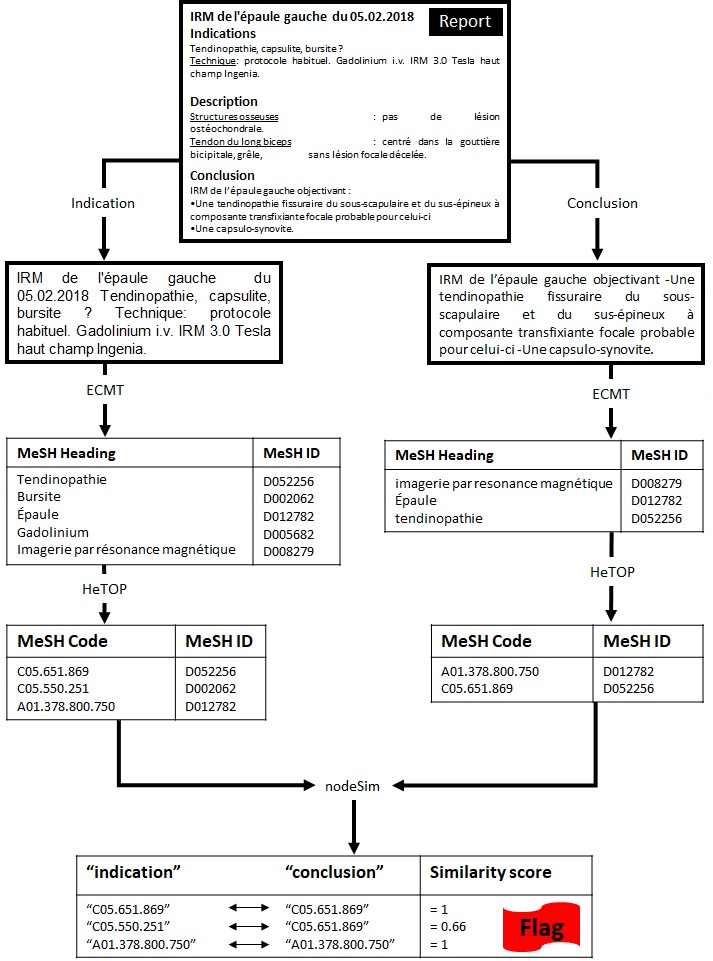
\includegraphics[scale=0.4]{FlowChart.jpg}
    \caption{Picture showing the processes followed in the developed prototype.}
    \label{fig:flowchart}
\end{figure}
%
\subsection{Prototype evaluation}
%
To evaluate the performance of the prototype, overall percentage concordance between indication and conclusion for all the radiology reports in the data set was automatically assessed.
Out of the 200 reports in the data set, a small subset was flagged by the prototype because the text corresponding to the \emph{conclusion} section was missing in these reports.
The \emph{conclusion} text from these reports was deliberately removed for testing this scenario.
Of the remaining reports, MeSH terms and codes for the anatomy and diseases were extracted from the indication and conclusion free-texts using ECMT and HeTOP.
Only 93 and 143 reports respectively contained MeSH terms corresponding to anatomy and disease.
Of these 143 reports, semantic similarity between indication and conclusion MeSH terms was obtained using nodeSim and total concordance was calculated.
To establish a ground truth, two expert radiologists repeated the above procedure manually and calculated the total concordance.

Upon total concordance assessment between the indication and conclusion, the prototype reported 45\% concordance for the anatomy information, while manual evaluation reported a 61\% concordance.
For disease information, the prototype reported 80\% concordance versus 88\% with the manual peer review.
Based on the ground truth, the algorithm accuracy for anatomy was 84\% and for disease 92\%.
It took the experienced radiologists about 1.5 hours to conduct manual quality checks, but the prototype did it in a matter of seconds.
%
\section{Discussion and Conclusion}
%
%Conclusion sections in SSRs should at least mention the investigated anatomical region and answer to the clinical indication for disease categories to avoid any misinterpretation and ensure comprehensiveness.
Reports with perfect match for the anatomy and disease MeSH terms between indication and conclusion correctly passed Q.C. Multiple reports were flagged when a particular anatomy term (e.g. knee) was mentioned in \emph{indication} but was missing in the \emph{conclusion}.
The prototype success, however, is subject to ability of ECMT to accurately extract the concepts from free texts and also upon availability of a particular concept in the MeSH vocabulary.
Currently, the prototype accounts only for the MeSH terminology, which lacks some radiology-specific terms~\cite{Demner-Fushman2015-ym}.
For example, a report mentioned \emph{epicondyle} in \emph{indications} section, but not in the \emph{conclusion} section.
This report passed Q.C. because no MeSH term corresponding to \emph{epicondyle} was identified from \emph{indications}.
Indeed, this term was absent in MeSH, but present in RadLex\footnote{http://www.radlex.org/RID/RID38647} and hence complementing the two can likely improve the results for the missed radiology terms.
However, only a part of RadLex is currently available in French.
In another instance, a disease term "D\'echirure" from free text indication was not identified by the ECMT, but a standardized, English counterpart for "D\'echirure" existed in MeSH as "Rupture".
This instance was reported to the ECMT team and the term was later added and semantically linked to its MeSH counterpart.
Overall prototype performance should also be improved with lexical standardization of disease terms in radiology reports, and further developments in the ECMT algorithm.

In conclusion, the automated prototype showed good performance compared to the expert radiologists for assessment of indication and conclusion concordance in the radiology reports.
It also reduces time and cost required for the quality control.
The prototype additionally identified the lack of systematic reporting of relevant anatomy information in the conclusion sections, a fact that can be highlighted in guidelines for radiologists.
%
%%%%% References %%%%%
\bibliographystyle{spiebib} 
%
\bibliography{MIE2020FullPaperRadiologyReports}
%
\end{document}